\documentclass[12pt,a4paper]{article}

\usepackage[utf8]{inputenc}
\usepackage[T1]{fontenc}
\usepackage{lmodern}
\usepackage{microtype}
\usepackage{graphicx}
\usepackage{amsmath}
\usepackage{amssymb}
\usepackage{geometry}
\usepackage{booktabs}
\usepackage{array}
\usepackage{tabularx}
\usepackage{hyperref}
\usepackage{fancyhdr}
\usepackage{listings}
\usepackage{xcolor}
\usepackage{float}
\usepackage{caption}
\usepackage{subcaption}
\usepackage{tikz}
\usetikzlibrary{arrows.meta,positioning,calc,decorations.pathreplacing}

\geometry{margin=1in}
\emergencystretch=1.5em
\setlength{\headheight}{14.5pt}
\pagestyle{fancy}
\fancyhf{}
\rhead{\thepage}
\lhead{Small-Signal Stability}

\hypersetup{
    colorlinks=true,
    linkcolor=blue,
    urlcolor=blue,
    citecolor=blue
}

\lstset{
    basicstyle=\ttfamily\small,
    keywordstyle=\color{blue},
    stringstyle=\color{red},
    commentstyle=\color{green!60!black},
    frame=single,
    breaklines=true,
    postbreak=\mbox{\textcolor{red}{$\hookrightarrow$}\space},
    showstringspaces=false
}

\newcommand{\dwr}{\Delta\omega_r}
\newcommand{\ddel}{\Delta\delta}
\newcommand{\dpsifd}{\Delta\psi_{fd}}

\title{\textbf{Small-Signal Stability Analysis and MATLAB
Simulation of a Single-Machine Infinite-Bus System}\\
\large Based on Kundur, \textit{Power System Stability and Control}, Chapter 12}
\author{Power System Stability --- Chapter 12 Study}
\date{May 31, 2026}

\raggedbottom

\begin{document}

\maketitle
\thispagestyle{empty}

\begin{abstract}
The single-machine infinite-bus (SMIB) system---a synchronous generator
connected through an equivalent reactance to an ideal constant-voltage,
constant-frequency bus---is the canonical model for studying rotor-angle
small-signal stability. \emph{Small-signal stability} is the ability of the
machine to remain in synchronism following a small disturbance; because the
disturbance is small, the system equations may be linearized about an operating
point and stability judged from the eigenvalues of the resulting state matrix.
This report analyzes the SMIB system at four levels of detail following Kundur,
\textit{Power System Stability and Control}, Chapter~12: the \emph{classical}
model (constant flux behind transient reactance), the \emph{field-circuit}
model (adding field-flux dynamics), the \emph{AVR} model (adding a thyristor
exciter and automatic voltage regulator), and the \emph{AVR\,+\,PSS} model
(adding a power system stabilizer). For each model the analysis builds the
linearized state-space representation, computes the eigenvalues, and evaluates
the damping ratio and oscillation frequency, with time-domain responses used to
confirm the eigenvalue predictions. The principal findings reproduce the
classical electromechanical swing frequency of $1.02$~Hz; show that
field-circuit dynamics contribute a small positive damping; demonstrate that a
high-gain AVR, in the presence of a negative $K_5$, \emph{reduces} damping
torque and can drive the swing mode unstable (eigenvalue $+0.504\pm j7.23$); and
confirm that a properly tuned PSS restores positive damping and returns the
swing mode to the stable left-half plane ($-1.005\pm j6.607$, $\zeta=0.15$). All
results agree with the corresponding Kundur Chapter~12 examples.
\end{abstract}
\newpage
\tableofcontents
\newpage

\section{Introduction}

Small-signal stability is the ability of a power system to maintain synchronism
when subjected to small disturbances such as incremental changes in load or
generation. Because such disturbances are small, the nonlinear system equations
may be linearized about a steady-state operating point. Stability is then
governed by the eigenvalues of the linearized state matrix: the system is
small-signal stable if and only if every eigenvalue has a negative real part.

The dominant concern for a synchronous generator connected to a large grid is
the \textit{electromechanical} or \textit{swing} mode---an oscillation of the
rotor against the rest of the system, typically in the range $0.1$--$2$~Hz. The
character of this mode is set by two torque components acting on the rotor: a
\textit{synchronizing} torque (in phase with the rotor-angle deviation $\ddel$)
and a \textit{damping} torque (in phase with the speed deviation $\dwr$).
Insufficient synchronizing torque produces a non-oscillatory (monotonic)
instability; insufficient damping torque produces a growing oscillation.

This report studies the four canonical SMIB models of Kundur Chapter~12. For
each, the linearized state matrix is assembled, its eigenstructure is computed,
and the result is interpreted physically and validated against the textbook.
The analysis is implemented and reproduced numerically in MATLAB; the
implementation is summarized in Section~\ref{sec:impl}, but the emphasis of the
report is the stability analysis itself.

\section{Objectives}

\begin{enumerate}
    \item Present the SMIB system and the meaning of small-signal stability for
          rotor-angle dynamics.
    \item Develop the linearized state-space model of the generator at four
          levels of detail: classical, field-circuit, AVR, and AVR\,+\,PSS.
    \item Derive the Heffron--Phillips $K$-constants from the fundamental
          $d$--$q$ machine parameters, including magnetic saturation.
    \item Evaluate stability through eigenvalues, damping ratios, and natural
          frequencies, and confirm the conclusions with time-domain responses.
    \item Demonstrate the effect of the AVR and the corrective action of the PSS
          on the swing mode, and validate every result against Kundur
          Chapter~12.
\end{enumerate}

\section{The Single-Machine Infinite-Bus System}
\label{sec:smib}

The single-machine infinite-bus (SMIB) system represents one synchronous
generator connected, through a transformer and transmission line of combined
equivalent reactance, to a very large power system. The large system is
idealized as an \emph{infinite bus}: a source of constant voltage magnitude,
constant frequency, and fixed phase angle that is unaffected by the behaviour of
the single machine. The infinite bus therefore serves as the angular and
frequency reference against which the generator's rotor swings.

In the classical representation the generator is modelled as a constant internal
voltage $E'\angle\delta$ behind the transient reactance $X_d'$, and the external
network as a series reactance $X_E$. The rotor angle $\delta$ is the angle of the
internal voltage relative to the infinite-bus voltage $E_B\angle 0^\circ$, as
shown in Figure~\ref{fig:smib}.

\begin{figure}[H]
\centering
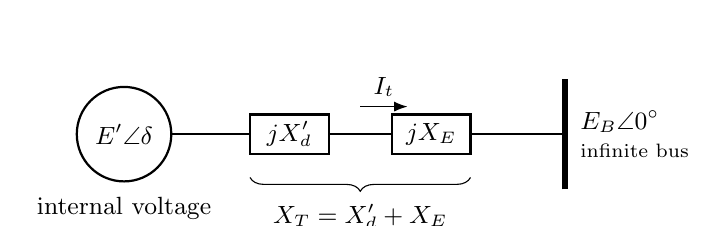
\begin{tikzpicture}[font=\small,>=Latex]
% Generator internal source
\draw[thick] (0,0) circle (0.6);
\node at (0,0) {$E'\angle\delta$};
\node[below=2pt] at (0,-0.6) {internal voltage};
% line out
\draw[thick] (0.6,0) -- (1.6,0);
% transient reactance
\draw[thick] (1.6,-0.25) rectangle (2.6,0.25);
\node at (2.1,0) {$jX_d'$};
% conductor
\draw[thick] (2.6,0) -- (3.4,0);
% external reactance
\draw[thick] (3.4,-0.25) rectangle (4.4,0.25);
\node at (3.9,0) {$jX_E$};
% conductor to bus
\draw[thick] (4.4,0) -- (5.6,0);
% infinite bus bar
\draw[line width=2pt] (5.6,-0.7) -- (5.6,0.7);
\node[right=2pt,align=left] at (5.6,0) {$E_B\angle 0^\circ$\\[-1pt]\scriptsize infinite bus};
% current arrow
\draw[->] (3.0,0.35) -- (3.6,0.35);
\node at (3.3,0.6) {$I_t$};
% total reactance brace
\draw[decorate,decoration={brace,amplitude=5pt,mirror}] (1.6,-0.55) -- (4.4,-0.55);
\node[below=6pt] at (3.0,-0.55) {$X_T = X_d' + X_E$};
\end{tikzpicture}
\caption{The single-machine infinite-bus system. The generator is represented by
a constant voltage $E'$ behind the transient reactance $X_d'$, connected through
the external reactance $X_E$ to an infinite bus of constant voltage
$E_B\angle 0^\circ$. The rotor angle $\delta$ is measured relative to the
infinite-bus reference; the total reactance is $X_T = X_d' + X_E$.}
\label{fig:smib}
\end{figure}

The SMIB system is used as the standard model for rotor-angle small-signal
stability because it isolates the electromechanical interaction between one
machine and the grid while remaining low-order enough to be analyzed in closed
form. It is the starting point for the linearized machine models developed in
the standard references on power system dynamics~\cite{kundur,anderson,sauer}.
The physical mechanisms it exposes---synchronizing and damping
torque, the destabilizing effect of high-gain voltage regulation, and the
corrective role of a power system stabilizer---carry over directly to machines
embedded in large multi-machine systems.

\section{Mathematical Modelling}
\label{sec:model}

\subsection{Power-Angle Relationship}

With the generator represented as $E'\angle\delta$ behind $X_d'$ and the network
as $X_E$, the air-gap (electrical) power delivered to the infinite bus is

\begin{equation}
P_e = \frac{E' E_B}{X_T}\sin\delta,
\qquad X_T = X_d' + X_E.
\label{eq:Pe}
\end{equation}

This is the power-angle curve: power transfer increases with rotor angle up to
$\delta = 90^\circ$. The slope of this curve at the operating point determines
how strongly the machine resists a change in angle---the synchronizing torque.

\subsection{Swing Equation}

The rotor motion is governed by the swing equation, which balances the
accelerating torque (mechanical input minus electrical output) against the rotor
inertia:

\begin{equation}
\frac{2H}{\omega_0}\frac{d^2\delta}{dt^2}
= T_m - T_e - K_D\,\Delta\omega_r,
\label{eq:swing}
\end{equation}

where $H$ is the inertia constant, $\omega_0 = 2\pi f_0$ the base electrical
speed, $K_D$ a damping coefficient, and $\Delta\omega_r$ the per-unit speed
deviation. The mechanical and electrical torques are nearly equal to the
corresponding powers in per unit near synchronous speed.

\subsection{Linearization}

For small deviations about the operating point $\delta_0$, the electrical power
of Eq.~\eqref{eq:Pe} is linearized as

\begin{equation}
\Delta P_e
= \left.\frac{\partial P_e}{\partial \delta}\right|_{\delta_0}\!\ddel
= \underbrace{\frac{E' E_B}{X_T}\cos\delta_0}_{K_S}\,\ddel
= K_S\,\ddel,
\label{eq:Ks}
\end{equation}

where $K_S$ is the \textit{synchronizing torque coefficient}. Substituting the
linearized power into the swing equation and writing the rotor angle and speed
deviations as states gives the state-space model below.

\subsection{State-Space Model: Classical}

With the generator represented by a constant voltage $E'$ behind $X_d'$, the
linearized swing equations are (Kundur Eq.~12.78):

\begin{equation}
\frac{d}{dt}
\begin{bmatrix} \dwr \\ \ddel \end{bmatrix}
=
\begin{bmatrix}
-\dfrac{K_D}{2H} & -\dfrac{K_S}{2H} \\[2ex]
\omega_0 & 0
\end{bmatrix}
\begin{bmatrix} \dwr \\ \ddel \end{bmatrix}
+
\begin{bmatrix} \dfrac{1}{2H} \\[2ex] 0 \end{bmatrix}
\Delta T_m.
\label{eq:classA}
\end{equation}

The undamped natural frequency and damping ratio follow from the characteristic
equation of Eq.~\eqref{eq:classA}:

\begin{equation}
\omega_n = \sqrt{\frac{K_S\,\omega_0}{2H}},
\qquad
\zeta = \frac{1}{2}\,\frac{K_D}{2H\,\omega_n}.
\label{eq:wn}
\end{equation}

\subsection{State-Space Model: Field-Circuit Dynamics}

Adding the field-winding flux linkage $\dpsifd$ as a third state captures the
slow demagnetizing effect of armature reaction. The state matrix becomes
(Kundur Eq.~12.116):

\begin{equation}
A_B =
\begin{bmatrix}
-\dfrac{K_D}{2H} & -\dfrac{K_1}{2H} & -\dfrac{K_2}{2H} \\[2ex]
\omega_0 & 0 & 0 \\[1ex]
0 & a_{32} & a_{33}
\end{bmatrix},
\end{equation}

where $K_1$ is the synchronizing torque coefficient at constant flux, $K_2$
relates electrical torque to field flux, and the field-equation entries are
$a_{32} = -K_3 K_4 / T_3$, $a_{33} = -1/T_3$. The constants $K_1$--$K_4$ and the
effective field time constant $T_3$ are derived from the $d$--$q$ parameters
(Section~\ref{sec:kderiv}).

\subsection{State-Space Model: Exciter and AVR}

A thyristor exciter (Kundur type ST1A) with gain $K_A$ and a terminal-voltage
transducer of time constant $T_R$ adds a fourth state $\Delta v_1$. Two further
constants are required: $K_5$ (the change in terminal voltage with rotor angle)
and $K_6$ (the change in terminal voltage with field flux). The field and
transducer rows are:

\begin{equation}
a_{34} = -\frac{K_3}{T_3}K_A,
\qquad
\dot{\Delta v_1} = \frac{K_5}{T_R}\ddel + \frac{K_6}{T_R}\dpsifd
- \frac{1}{T_R}\Delta v_1.
\end{equation}

The field-flux response to a rotor-angle perturbation, including exciter action,
is (Kundur Eq.~12.144 with $G_{ex}(s)=K_A$):

\begin{equation}
\frac{\dpsifd}{\ddel}(s) =
\frac{-K_3\bigl[K_4(1+sT_R) + K_5 K_A\bigr]}
     {(1+sT_3)(1+sT_R) + K_3 K_6 K_A}.
\label{eq:psifd}
\end{equation}

Evaluating $K_2 \cdot \dpsifd/\ddel$ at $s = j\omega$ (the swing frequency)
decomposes the field/AVR torque into a synchronizing part (real) and a damping
part (imaginary, scaled by $\omega_0/\omega$). With $K_5<0$, increasing $K_A$
raises synchronizing torque but reduces damping torque---the central trade-off
of high-gain AVRs.

\subsection{State-Space Model: Power System Stabilizer}

The PSS restores damping by injecting a supplementary signal derived from
$\dwr$ through a washout and lead-lag compensator (Kundur Eq.~12.151):

\begin{equation}
G_{PSS}(s) = K_{STAB}\,
\frac{sT_w}{1+sT_w}\,
\frac{1+sT_1}{1+sT_2}.
\end{equation}

The washout state $\Delta v_2$ and lead-lag output $\Delta v_s$ extend the model
to six states. The stabilizer output enters the exciter summing junction, adding
phase lead that converts the AVR's negative damping back to positive.

\subsection{Summary of the Four Models}

The four models form a hierarchy of increasing detail. Each adds states that
capture an additional physical effect, as summarized in
Table~\ref{tab:statevec}.

\begin{table}[H]
\centering
\caption{State-space model summary. Each model augments the previous one with
states representing an additional physical subsystem.}
\label{tab:statevec}
\begin{tabular}{@{}l l p{5.6cm}@{}}
\toprule
Model & State vector & Purpose \\
\midrule
Classical    & $[\dwr,\ \ddel]^T$
             & Basic electromechanical swing mode \\
Field-circuit & $[\dwr,\ \ddel,\ \dpsifd]^T$
             & Adds field-flux (rotor circuit) dynamics \\
AVR          & $[\dwr,\ \ddel,\ \dpsifd,\ \Delta v_1]^T$
             & Adds exciter / voltage-regulator effect \\
AVR + PSS    & $[\dwr,\ \ddel,\ \dpsifd,\ \Delta v_1,\ \Delta v_2,\ \Delta v_s]^T$
             & Adds supplementary damping through the stabilizer \\
\bottomrule
\end{tabular}
\end{table}

\subsection{Eigen-Analysis}

For state matrix $A$ with eigenvalue $\lambda = \sigma \pm j\omega$:

\begin{equation}
\zeta = \frac{-\sigma}{\sqrt{\sigma^2+\omega^2}},
\qquad
f = \frac{|\omega|}{2\pi}\ \text{Hz}.
\end{equation}

The right eigenvector gives the \textit{mode shape} (relative activity and phase
of each state in the mode); the participation factor
$p_{ki} = |v_{ki}|\,|w_{ik}|$ measures the contribution of state $k$ to mode
$i$, dimensionless and independent of units.

\section{Small-Signal Stability Analysis Procedure}
\label{sec:procedure}

The stability of each model is evaluated by the following systematic procedure,
applied identically to all four model levels:

\begin{enumerate}
    \item \textbf{Operating point.} Solve the steady-state network and machine
          equations for the rotor angle $\delta_0$, the internal voltage $E'$,
          and the $d$--$q$ currents and fluxes.
    \item \textbf{$K$-constants.} Derive (or, where the textbook supplies them,
          adopt) the Heffron--Phillips constants $K_1$--$K_6$ and the field time
          constant $T_3$ from the operating point and machine parameters.
    \item \textbf{State matrix.} Assemble the linearized state matrix $A$ for
          the chosen model level.
    \item \textbf{Eigenvalues.} Compute the eigenvalues $\lambda_i = \sigma_i \pm
          j\omega_i$ of $A$.
    \item \textbf{Stability test.} Determine stability from the real parts: the
          system is stable if and only if $\sigma_i < 0$ for all $i$.
    \item \textbf{Damping and frequency.} For each oscillatory mode compute the
          damping ratio $\zeta_i$ and frequency $f_i$.
    \item \textbf{Time-domain validation.} Confirm the eigenvalue prediction
          with the time response (rotor angle, speed, and electrical power) to a
          small disturbance.
\end{enumerate}

\section{Derivation of the $K$-Constants from $d$--$q$ Parameters}
\label{sec:kderiv}

The $K$-constants of the field-circuit model are computed from the fundamental
machine parameters rather than supplied directly. The procedure follows Kundur
Example 12.3:

\begin{enumerate}
    \item \textbf{Saturation.} The total air-gap flux $\psi_{at}$ at the
          operating point sets the saturation factors. Above the threshold
          $\psi_{T1}$, the incremental saturated inductance uses
          $K_{sd}^{incr} = 1/(1 + B_{sat}\psi_I)$ with
          $\psi_I = A_{sat}\exp[B_{sat}(\psi_{at}-\psi_{T1})]$.
    \item \textbf{Operating point.} The internal angle is obtained directly as
          $\delta_0 = \operatorname{atan2}(E_{Bd0}, E_{Bq0})$, from which the
          $d$- and $q$-axis currents $i_{d0}, i_{q0}$, the field current
          $i_{fd0}$, and the field voltage $E_{fd0} = L_{adu}\,i_{fd0}$ follow.
    \item \textbf{Network-coupling coefficients.} The constants $m_1, n_1, m_2,
          n_2$ (Kundur Eqs.~12.106--12.108) couple the rotor-angle and
          field-flux perturbations to the $d$--$q$ currents. A subtlety
          confirmed during validation: $m_2, n_2$ use the \emph{incremental}
          $L_{ads}$ (not the parallel $L_{ads}'$).
    \item \textbf{$K$-constants.} $K_1, K_2$ are assembled from
          $m_1, n_1, m_2, n_2$ and the operating-point fluxes; $K_4$ satisfies
          $a_{32} = -(\omega_0 R_{fd}/L_{adu})K_4$ (note $L_{adu}$, not
          $L_{fd}$); $T_3 = -1/a_{33}$.
\end{enumerate}

\subsection{Physical Meaning of the $K$-Constants}

The six Heffron--Phillips constants each quantify one linearized coupling in the
machine. Their physical meanings are summarized in Table~\ref{tab:kmeaning}.

\begin{table}[H]
\centering
\caption{Physical meaning of the Heffron--Phillips $K$-constants.}
\label{tab:kmeaning}
\begin{tabular}{@{}c p{11cm}@{}}
\toprule
Constant & Physical meaning \\
\midrule
$K_1$ & Change in electrical torque for a change in rotor angle at constant flux
        (synchronizing torque) \\
$K_2$ & Change in electrical torque for a change in field flux linkage \\
$K_3$ & Field-circuit gain factor (impedance factor of the field loop) \\
$K_4$ & Demagnetizing effect of a change in rotor angle on the field flux \\
$K_5$ & Change in terminal voltage for a change in rotor angle \\
$K_6$ & Change in terminal voltage for a change in field flux linkage \\
\bottomrule
\end{tabular}
\end{table}

The constant $K_5$ is pivotal. Under heavy load and high external reactance
$K_5$ becomes \emph{negative}, meaning a rotor-angle increase \emph{lowers} the
terminal voltage. A high-gain AVR then responds with a field-voltage action that
is out of phase with the rotor swing, producing negative damping torque. This
single sign change explains why a regulator intended to improve voltage control
can degrade rotor-angle damping (Section~\ref{sec:avr}) and motivates the PSS
(Section~\ref{sec:pss}).

Table~\ref{tab:kderiv} confirms the derived values against Example 12.3.

\section{MATLAB Implementation}
\label{sec:impl}

The analysis is carried out by a small set of MATLAB routines: case definitions
hold the machine, network, and operating data together with the textbook golden
references; an operating-point and $K$-constant layer derives the linearization;
a state-matrix builder assembles models A--D; and an eigen-analysis routine
returns eigenvalues, damping ratios, mode shapes, and participation factors. A
standalone runner executes all four models end-to-end and produces the figures
of Section~\ref{sec:figs}. Table~\ref{tab:impl} lists the components.

\begin{table}[H]
\centering
\caption{MATLAB components used to produce the results in this report.}
\label{tab:impl}
\begin{tabular}{@{}lll@{}}
\toprule
Component & File & Role \\
\midrule
Cases          & \texttt{+cases/case\_kundur\_smib\_*.m} & parameters + golden refs \\
Classical init & \texttt{+smib/smib\_classical\_init.m}  & $\delta_0$, $E'$, $K_S$ \\
$d$--$q$ init  & \texttt{+smib/smib\_dq\_init.m}         & operating point, saturation \\
$K$-constants  & \texttt{+smib/smib\_k\_constants.m}     & derive $K_1$--$K_4$, $T_3$ \\
Torque decomp. & \texttt{+smib/smib\_torque\_components.m} & $K_S$, $K_D$ vs $K_A$ \\
State matrix   & \texttt{+smib/smib\_build\_state\_matrix.m} & models A/B/C/D \\
Eigen-analysis & \texttt{+smib/smib\_analyze.m}          & $\lambda$, $\zeta$, mode shape \\
Plots          & \texttt{internal/plotting/smib\_plot\_*.m} & figures \\
Runner         & \texttt{run\_smib\_example.m}           & end-to-end analysis \\
\bottomrule
\end{tabular}
\end{table}

\section{Worked Examples and Validation}

This section analyzes four worked cases from Kundur Chapter~12. For each, the
problem data are stated first, then the analysis procedure of
Section~\ref{sec:procedure} is applied, and finally the computed result is
compared against the textbook value.

\subsection{Example 12.2 --- Classical Model}

\textbf{Problem (Kundur Ex.\ 12.2, pp.\ 732--737).} A 2220~MVA, 24~kV, 60~Hz
generator with inertia $H=3.5$ and transient reactance $X_d'=0.30$~pu delivers
$P=0.9$~pu, $Q=0.3$~pu (overexcited) at a terminal voltage
$E_t = 1.0\angle 36^\circ$~pu. The external reactance to the infinite bus is
$X_E = 0.65$~pu and the infinite-bus voltage is $E_B = 0.995\angle 0^\circ$~pu.
Find the operating point, the synchronizing torque coefficient $K_S$, and the
swing-mode eigenvalues for $K_D = 0, 10, -10$.

\textbf{Solution}
\begin{enumerate}
\item Terminal current from $S = E_t I_t^{*}$:
      \[ I_t = \left(\frac{P+jQ}{E_t}\right)^{\!*} = 0.9487\angle 17.57^\circ
         = 0.9045 + j0.2863 \ \text{pu}. \]
\item Internal voltage behind $X_d'$ (armature resistance neglected):
      \[ E' = E_t + jX_d' I_t = 1.1229\angle 49.91^\circ \ \text{pu}. \]
\item Rotor angle relative to the infinite bus:
      $\delta_0 = \angle E' - \angle E_B = 49.91^\circ$.
\item Total reactance $X_T = X_d' + X_E = 0.30 + 0.65 = 0.95$~pu.
\item Synchronizing coefficient (Eq.~\ref{eq:Ks}):
      \[ K_S = \frac{|E'|\,|E_B|}{X_T}\cos\delta_0
             = \frac{1.1229 \times 0.995}{0.95}\cos 49.91^\circ = 0.7574. \]
\item Undamped natural frequency (Eq.~\ref{eq:wn}) with
      $\omega_0 = 2\pi(60) = 376.99$~rad/s:
      \[ \omega_n = \sqrt{\frac{K_S\,\omega_0}{2H}}
         = \sqrt{\frac{0.7574 \times 376.99}{7}} = 6.387\ \text{rad/s}
         = 1.0165\ \text{Hz}. \]
\end{enumerate}

\begin{table}[H]
\centering
\caption{Example 12.2 --- computed vs.\ textbook golden values.}
\label{tab:modelA}
\begin{tabular}{@{}lrr@{}}
\toprule
Quantity & Computed & Golden \\
\midrule
$\delta_0$ (deg)        & 49.91 & 49.92 \\
$|E'|$ (pu)             & 1.123 & 1.123 \\
$X_T$ (pu)              & 0.950 & 0.950 \\
$K_S$                   & 0.7574 & 0.757 \\
$f_n$ (Hz)              & 1.0165 & 1.0165 \\
$\lambda$ ($K_D{=}0$)   & $\pm j6.387$ & $\pm j6.39$ \\
$\lambda$ ($K_D{=}10$)  & $-0.714\pm j6.347$ & $-0.714\pm j6.35$ \\
$\zeta$ ($K_D{=}10$)    & 0.112 & 0.112 \\
$\lambda$ ($K_D{=}{-}10$) & $+0.714\pm j6.347$ & $+0.714\pm j6.36$ \\
\bottomrule
\end{tabular}
\end{table}

With $K_D=0$ the mode is undamped (purely imaginary eigenvalues, $f=1.02$~Hz);
positive damping moves it into the left-half plane, and negative damping into
the right-half plane (instability). The root locus as $K_D$ is swept is shown in
Figure~\ref{fig:rootlocus}; the rotor-angle and speed responses for $K_D=10$ in
Figure~\ref{fig:step}; and the corresponding electrical-power response in
Figure~\ref{fig:power}.

\subsection{Example 12.3 --- Field-Circuit Dynamics}

\textbf{Problem (Kundur Ex.\ 12.3, pp.\ 753--757).} The same machine and
operating point as Example 12.2, but now modelled with field-circuit dynamics
and magnetic saturation. The fundamental machine parameters (pu, machine base)
are listed in Table~\ref{tab:Bgiven}. Derive the Heffron--Phillips constants
$K_1$--$K_4$ and $T_3$ \emph{from these parameters}, assemble the $3\times3$
state matrix, and find the eigenvalues.

\begin{table}[H]
\centering
\caption{Example 12.3 --- given machine and network data.}
\label{tab:Bgiven}
\begin{tabular}{@{}llll@{}}
\toprule
Parameter & Value & Parameter & Value \\
\midrule
$L_{adu}$ & 1.65 & $R_{fd}$  & 0.0006 \\
$L_{aqu}$ & 1.60 & $A_{sat}$ & 0.031 \\
$L_l$     & 0.16 & $B_{sat}$ & 6.93 \\
$R_a$     & 0.003 & $\psi_{T1}$ & 0.80 \\
$L_{fd}$  & 0.153 & $X_E$ & 0.65 \\
$H$       & 3.5 & $K_D$ & 0 \\
\bottomrule
\end{tabular}
\end{table}
\newpage
\textbf{Solution}
\begin{enumerate}
\item \textit{Saturation.} Air-gap flux
      $\psi_{at} = |E_t + (R_a + jL_l)I_t| = 1.0604$. Since
      $\psi_{at}>\psi_{T1}$,
      $\psi_I = A_{sat}e^{B_{sat}(\psi_{at}-\psi_{T1})} = 0.1884$, giving the
      total and incremental saturation factors $K_{sd}=0.8491$,
      $K_{sd}^{incr}=0.4337$. Hence the saturated mutual inductances
      $L_{ads}=0.8491(1.65)=1.4011$, $L_{aqs}=1.3586$, and the incremental
      $L_{ads}^{incr}=0.7156$.
\item \textit{Internal angle and currents.}
      $\delta_i = \angle\!\left[E_t + (R_a + jX_{qs})I_t\right] = 43.13^\circ$,
      from which $i_{d0}=0.8342$, $i_{q0}=0.4518$, $e_{d0}=0.6836$,
      $e_{q0}=0.7299$.
\item \textit{Rotor angle and field.} Resolving onto the infinite-bus frame
      gives $E_{Bd0}=0.9773$, $E_{Bq0}=0.1876$, so
      $\delta_0 = \operatorname{atan2}(E_{Bd0},E_{Bq0}) = 79.13^\circ$. The field
      current $i_{fd0}=1.4514$ yields $E_{fd0}=L_{adu}i_{fd0}=2.395$.
\item \textit{Coupling coefficients} (Eqs.~12.106--12.108):
      $m_1 = 1.0436$, $n_1 = 0.1268$, $m_2 = 0.8801$, $n_2 = 0.00176$.
\item \textit{$K$-constants:} $K_1 = 0.7643$, $K_2 = 0.8649$, $K_3 = 0.323$,
      $K_4 = 1.4187$, and $T_3 = -1/a_{33} = 2.356$~s.
\end{enumerate}

The resulting state matrix and its eigenvalues are:
\begin{equation}
A_B =
\begin{bmatrix}
0 & -0.1092 & -0.1236 \\
376.99 & 0 & 0 \\
0 & -0.1945 & -0.4244
\end{bmatrix},
\qquad
\lambda =
\begin{cases}
-0.110 \pm j6.411 & \text{(swing)} \\
-0.205 & \text{(field)}
\end{cases}
\end{equation}

\begin{table}[H]
\centering
\caption{Example 12.3 --- derived constants and eigenvalues vs.\ golden.}
\label{tab:kderiv}
\begin{tabular}{@{}lrr@{}}
\toprule
Quantity & Derived & Golden \\
\midrule
$\delta_0$ (deg) & 79.13 & 79.13 \\
$E_{fd0}$ (pu)   & 2.395 & 2.395 \\
$m_1$ & 1.0436 & 1.0437 \\
$n_1$ & 0.1268 & 0.1268 \\
$m_2$ & 0.8801 & 0.8802 \\
$K_1$            & 0.7643 & 0.7643 \\
$K_2$            & 0.8649 & 0.8649 \\
$K_4$            & 1.4187 & 1.4187 \\
$T_3$ (s)        & 2.356 & 2.365 \\
swing $\lambda$  & $-0.110\pm j6.411$ & $-0.110\pm j6.41$ \\
field $\lambda$  & $-0.205$ & $-0.204$ \\
\bottomrule
\end{tabular}
\end{table}

The field circuit introduces a small positive damping (swing-mode
$\zeta\approx0.017$) and a non-oscillatory field mode near $-0.204$. The
participation factors confirm the physical identity of each mode: the swing mode
is $49\%$ $\dwr$ + $49\%$ $\ddel$ with only $1.7\%$ $\dpsifd$, whereas the field
mode is $99.8\%$ $\dpsifd$ (Table~\ref{tab:partic}, visualized in
Figure~\ref{fig:modeshape}).

\begin{table}[H]
\centering
\caption{Example 12.3 --- participation-factor matrix (state $\times$ mode).}
\label{tab:partic}
\begin{tabular}{@{}lrr@{}}
\toprule
State & Swing mode ($-0.110\pm j6.41$) & Field mode ($-0.205$) \\
\midrule
$\dwr$    & 0.492 & 0.001 \\
$\ddel$   & 0.492 & 0.001 \\
$\dpsifd$ & 0.017 & 0.998 \\
\bottomrule
\end{tabular}
\end{table}

\subsection{Table 12.1 --- Effect of the AVR}
\label{sec:avr}

\textbf{Problem (Kundur Sec.\ 12.4, pp.\ 762--765).} For a machine with
$K_1=1.591$, $K_2=1.5$, $K_3=0.333$, $K_4=1.8$, $K_5=-0.12$, $K_6=0.3$,
$T_3=1.91$~s, $H=3.0$, and a thyristor exciter of transducer time constant
$T_R=0.02$~s, evaluate how the synchronizing and damping torque components
contributed by the field/AVR loop vary as the exciter gain $K_A$ is increased.

\textbf{Method.} The field-flux response to a rotor-angle perturbation is given
by Eq.~\ref{eq:psifd}. The contribution to electrical torque is
$\Delta T_e = K_2\,\dpsifd$. Evaluating $K_2\cdot\dpsifd/\ddel$ at $s=j\omega$
(with $\omega \approx 10$~rad/s, the swing frequency) and separating real and
imaginary parts gives the synchronizing component $K_S(\dpsifd)$ and the damping
component $K_D(\dpsifd) = \operatorname{Im}(\cdot)\,\omega_0/\omega$.

\begin{table}[H]
\centering
\caption{Table 12.1 --- torque components vs.\ AVR gain $K_A$ ($\omega=10$~rad/s).}
\label{tab:modelC}
\begin{tabular}{@{}rrrrr@{}}
\toprule
$K_A$ & $K_S(\dpsifd)$ & golden & $K_D(\dpsifd)$ & golden \\
\midrule
0   & $-0.0025$ & $-0.0025$ & $+1.770$  & $+1.772$ \\
15  & $-0.0093$ & $-0.0093$ & $+0.024$  & $+0.024$ \\
25  & $-0.0098$ & $-0.0098$ & $-1.165$  & $-1.166$ \\
200 & $+0.2801$ & $+0.2804$ & $-12.271$ & $-12.272$ \\
\bottomrule
\end{tabular}
\end{table}

With $K_5<0$ the damping coefficient crosses zero near $K_A\approx15$ and becomes
strongly negative at high gain: the AVR improves synchronizing torque at the
expense of damping (Figure~\ref{fig:torque}). Using the Example 12.6 $K$-set, a
full eigen-analysis of the 4-state AVR model at $K_A=200$ confirms an unstable
swing mode at $+0.504\pm j7.23$.

\subsection{Example 12.6 --- AVR plus PSS}
\label{sec:pss}

\textbf{Problem (Kundur Ex.\ 12.6, pp.\ 776--778).} For the Example 12.3 machine
with the high-gain AVR ($K_A=200$) that destabilizes the rotor mode, design a
power system stabilizer with $K_{STAB}=9.5$, washout $T_w=1.4$~s, and lead-lag
$T_1=0.154$~s, $T_2=0.033$~s. Show that the PSS restores stability.

\textbf{Result.} The full 6-state eigenvalues with the PSS in service are
\[
\lambda = \{\,-39.10,\ -1.005\pm j6.607,\ -0.739,\ -19.80\pm j12.82\,\},
\]
all in the left-half plane. The swing mode moves from $+0.504\pm j7.23$ (AVR
only, $\zeta=-0.07$) to $-1.005\pm j6.607$ ($\zeta=+0.15$); the migration on the
complex plane is shown in Figure~\ref{fig:eigcmp}.

\begin{table}[H]
\centering
\caption{Example 12.6 --- swing mode with and without PSS at $K_A=200$.}
\label{tab:modelD}
\begin{tabular}{@{}lrrrc@{}}
\toprule
Configuration & swing $\lambda$ & golden & $\zeta$ & stable \\
\midrule
AVR only      & $+0.504\pm j7.232$ & $+0.504\pm j7.23$ & $-0.070$ & no \\
AVR + PSS     & $-1.005\pm j6.607$ & $-1.005\pm j6.607$ & $+0.150$ & yes \\
\bottomrule
\end{tabular}
\end{table}

Adding the PSS converts the unstable AVR-only swing mode into a well-damped mode
($\zeta=0.15$), matching Example 12.6 exactly. The well-damped exciter mode
($-19.8\pm j12.8$, $\zeta=0.84$) and the washout-related real mode ($-0.739$)
also agree with the textbook.

\section{Figures and Interpretation}
\label{sec:figs}

\begin{figure}[H]
\centering
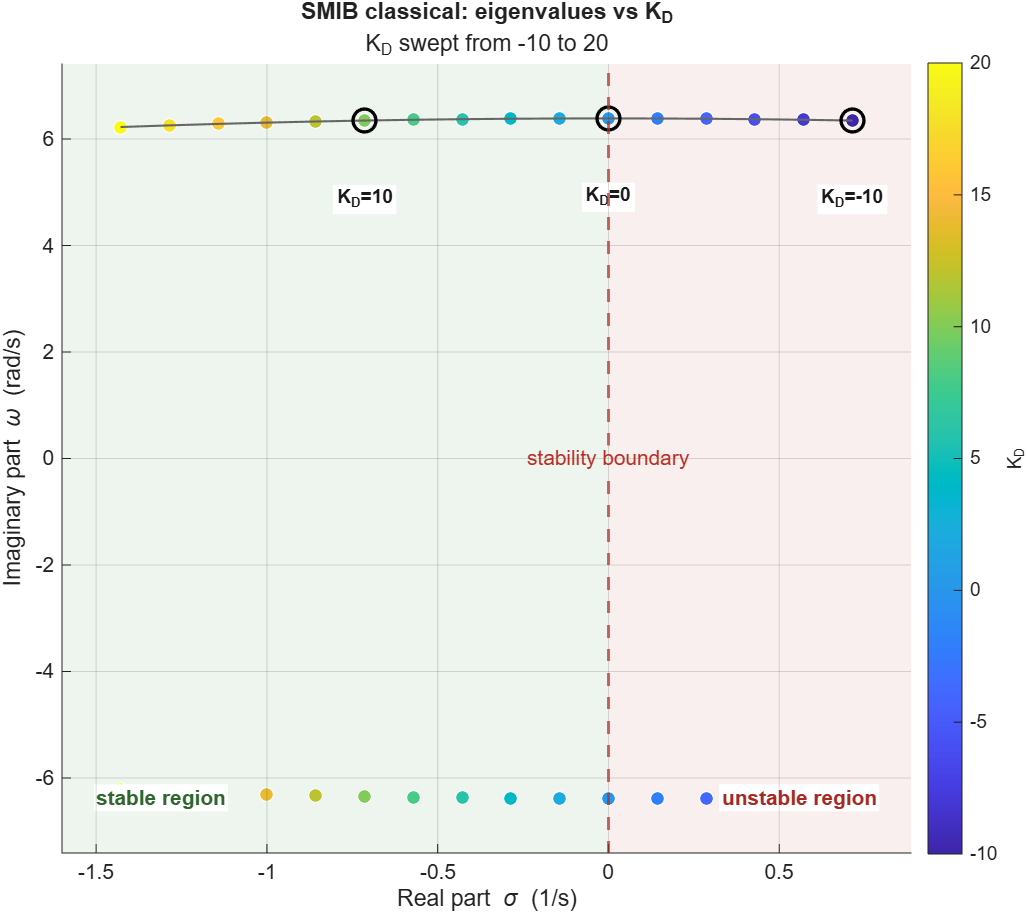
\includegraphics[width=0.85\textwidth]{figures/01_root_locus.png}
\caption{Eigenvalue plot / root locus of the classical SMIB model as the damping
coefficient $K_D$ is swept from $-10$ to $+20$. The shaded left-half plane is
the stable region and the right-half plane the unstable region; the dashed
imaginary axis is the stability boundary ($\sigma=0$). Increasing positive
damping $K_D$ shifts the swing eigenvalues leftward into the stable region,
while negative damping shifts them rightward into the unstable region; the
marked points correspond to $K_D=-10$, $0$, and $+10$.}
\label{fig:rootlocus}
\end{figure}

\begin{figure}[H]
\centering
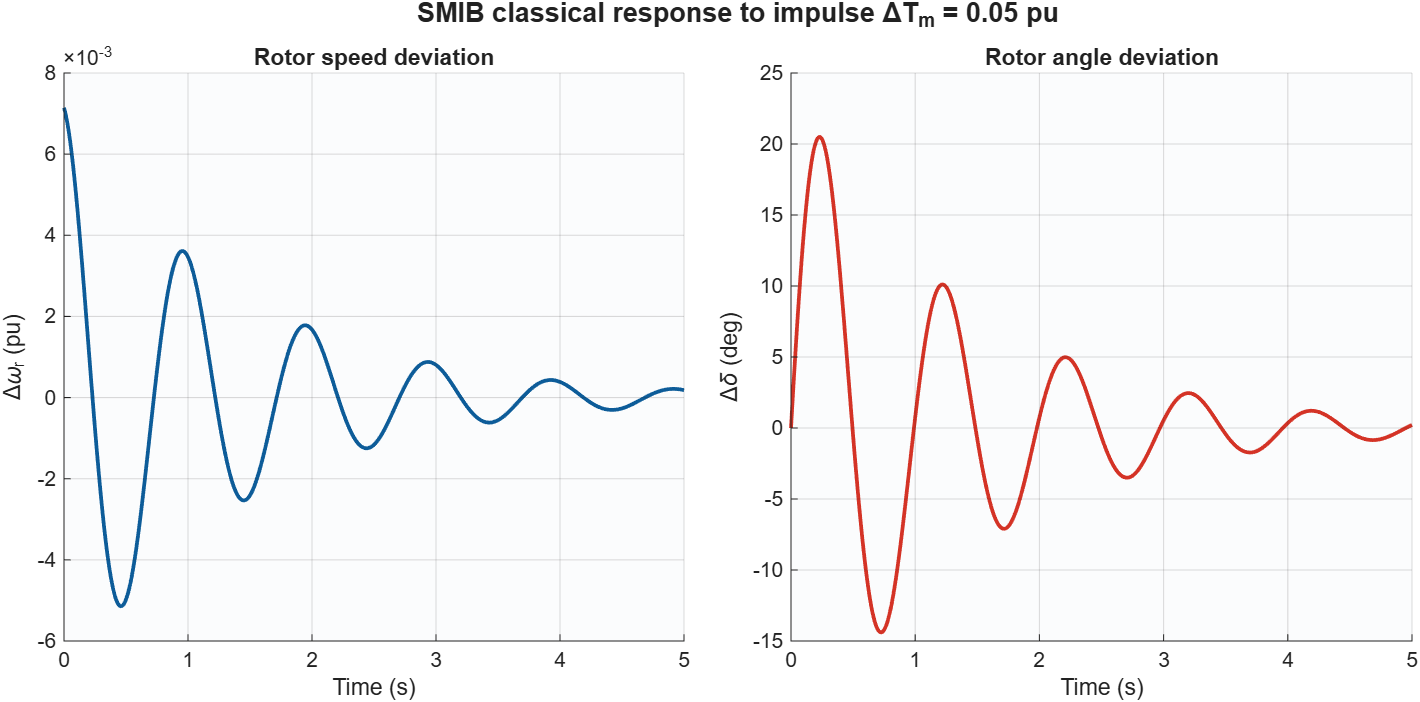
\includegraphics[width=0.9\textwidth]{figures/02_step_response.png}
\caption{Time-domain response of the classical model ($K_D=10$) to a small
torque disturbance. Left: rotor speed deviation $\dwr$, which decays to zero as
the rotor returns to synchronous speed. Right: rotor angle deviation $\ddel$,
whose decaying $\sim1$~Hz oscillation ($\zeta=0.112$) shows that the generator
remains in synchronism with the infinite bus.}
\label{fig:step}
\end{figure}

\begin{figure}[H]
\centering
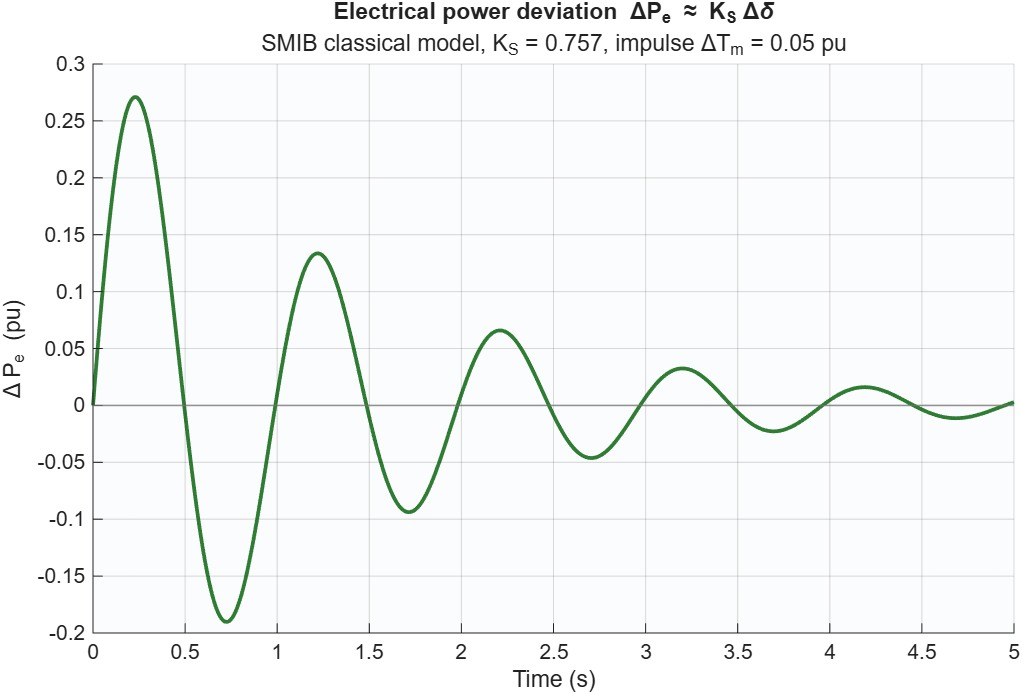
\includegraphics[width=0.7\textwidth]{figures/05_power_response.png}
\caption{Electrical power response of the classical model ($K_D=10$) to the same
disturbance, computed as $\Delta P_e \approx K_S\,\ddel$. The decaying power
oscillation confirms that the machine settles back to steady power transfer with
the infinite bus---the time-domain signature of a small-signal stable system.}
\label{fig:power}
\end{figure}

\begin{figure}[H]
\centering
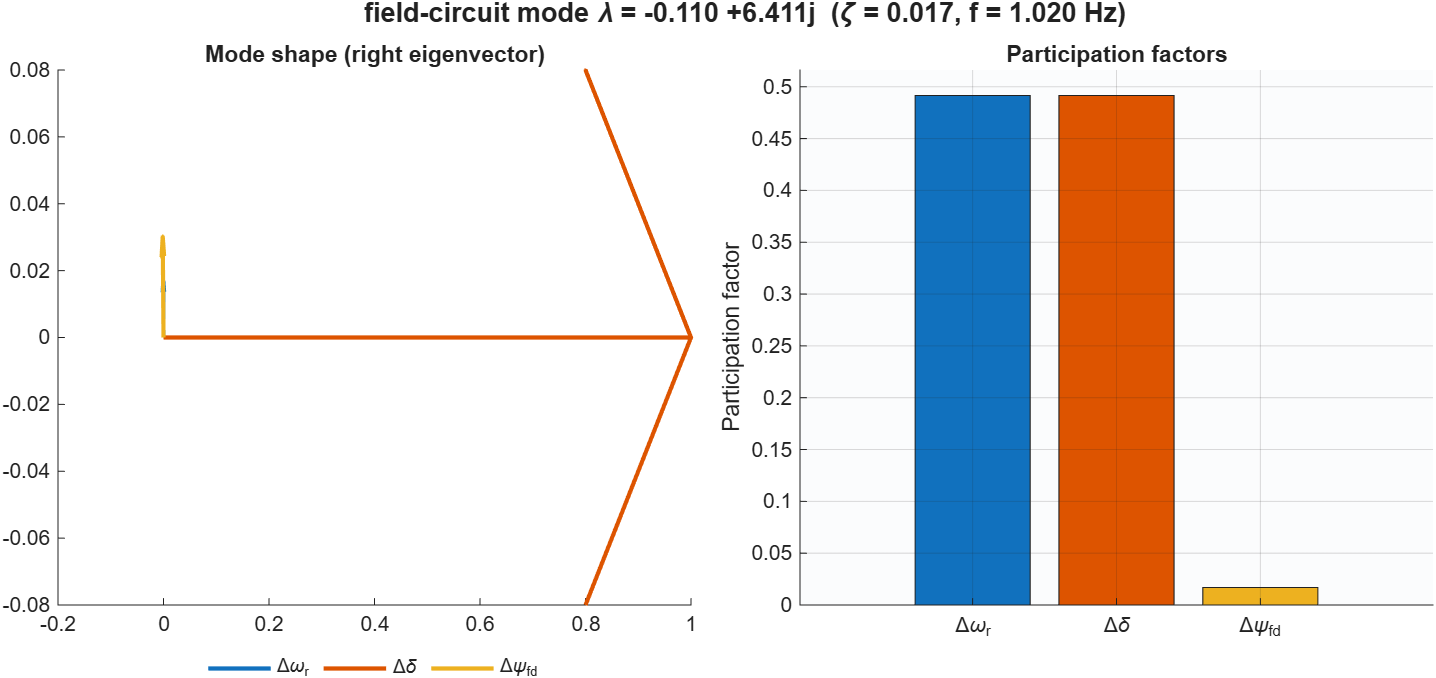
\includegraphics[width=0.9\textwidth]{figures/03_mode_shape.png}
\caption{Mode shape (left) and participation factors (right) of the
field-circuit swing mode. The rotor states $\dwr$ and $\ddel$ dominate the
electromechanical mode; the field flux $\dpsifd$ contributes negligibly,
confirming the modal identification of Table~\ref{tab:partic}.}
\label{fig:modeshape}
\end{figure}

\begin{figure}[H]
\centering
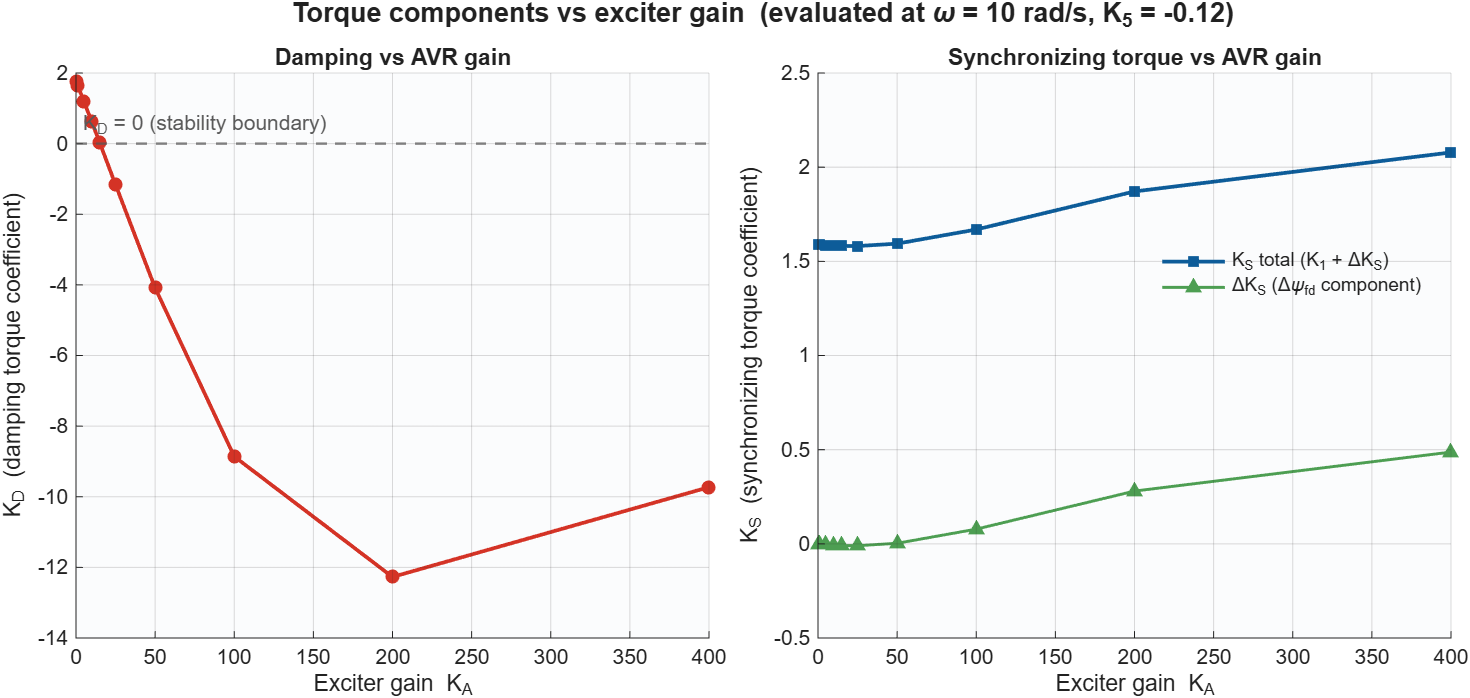
\includegraphics[width=0.9\textwidth]{figures/04_torque_vs_ka.png}
\caption{Damping (left) and synchronizing (right) torque coefficients versus AVR
gain $K_A$. With $K_5<0$, raising the gain increases the synchronizing torque
$K_S$ but drives the damping torque $K_D$ negative, reproducing Kundur Table
12.1. Negative damping is the mechanism by which a high-gain AVR destabilizes the
swing mode.}
\label{fig:torque}
\end{figure}

\begin{figure}[H]
\centering
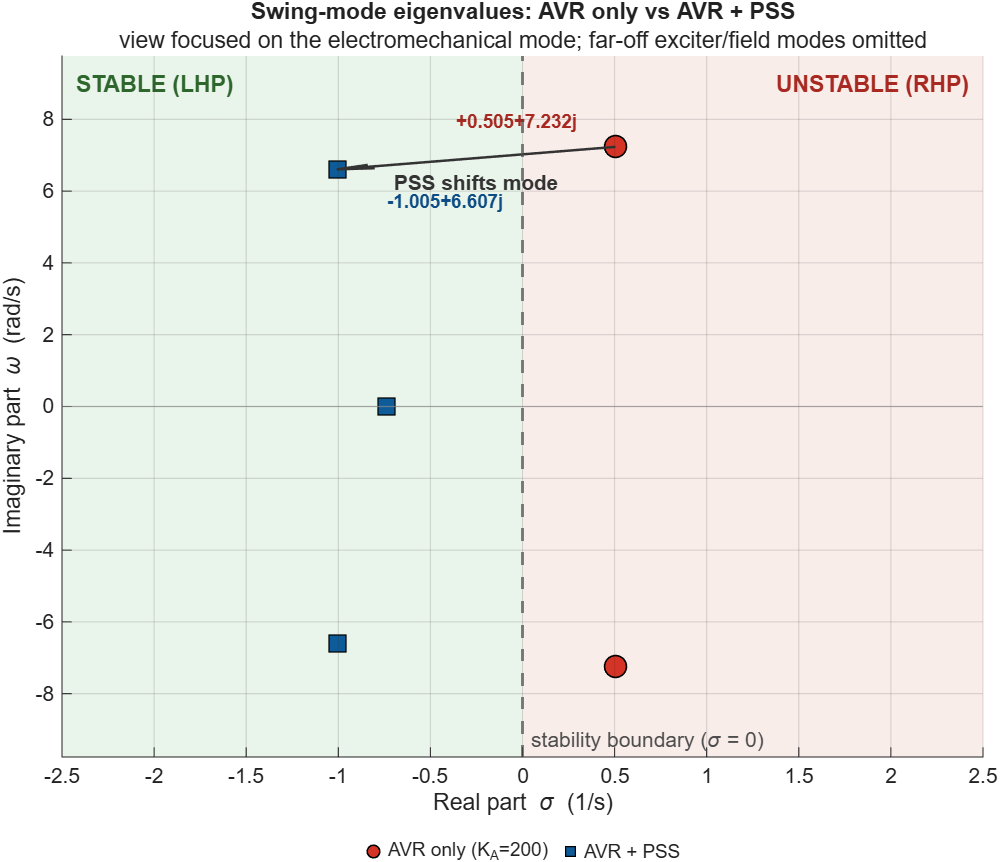
\includegraphics[width=0.8\textwidth]{figures/06_eig_comparison.png}
\caption{Swing-mode eigenvalues with AVR only (right-half plane,
$+0.504\pm j7.23$, unstable) and with AVR\,+\,PSS (left-half plane,
$-1.005\pm j6.607$, stable) at $K_A=200$. The PSS moves the electromechanical
mode across the stability boundary into the stable region. The view is focused
on the swing mode; the far-off exciter and field modes lie outside the frame.}
\label{fig:eigcmp}
\end{figure}

\noindent
Table~\ref{tab:figinterp} summarizes how each figure is read in stability terms.

\begin{table}[H]
\centering
\caption{Interpretation of the figures in small-signal stability terms.}
\label{tab:figinterp}
\renewcommand{\arraystretch}{1.3}
\newcolumntype{Y}{>{\raggedright\arraybackslash}X}
\begin{tabularx}{\textwidth}{@{}>{\raggedright\arraybackslash\hyphenpenalty=10000\exhyphenpenalty=10000}p{4.3cm}Y Y@{}}
\toprule
\textbf{Figure} & \textbf{What it shows} & \textbf{Stability interpretation} \\
\midrule
Eigenvalue plot / root locus (Fig.~\ref{fig:rootlocus})
 & Movement of eigenvalues as $K_D$ varies
 & Left-half plane $\Rightarrow$ stable; right-half plane $\Rightarrow$ unstable \\
Rotor angle response (Fig.~\ref{fig:step}, right)
 & Oscillation of $\ddel$
 & Decaying oscillation $\Rightarrow$ synchronism is maintained \\
Rotor speed response (Fig.~\ref{fig:step}, left)
 & Oscillation of $\dwr$
 & Return to zero $\Rightarrow$ speed returns to synchronous \\
Electrical power response (Fig.~\ref{fig:power})
 & Oscillation of $\Delta P_e$
 & Decaying power oscillation $\Rightarrow$ stable power transfer \\
AVR gain effect (Fig.~\ref{fig:torque})
 & $K_S$ and $K_D$ versus $K_A$
 & High gain raises $K_S$ but can reduce $K_D$ \\
AVR vs PSS eigenvalues (Fig.~\ref{fig:eigcmp})
 & Swing mode before and after PSS
 & PSS moves the mode to the stable left-half plane \\
\bottomrule
\end{tabularx}
\end{table}

\section{Discussion}
\label{sec:discussion}

The four models together tell a single, coherent story about rotor-angle
small-signal stability.

\begin{itemize}
    \item \textbf{Classical model.} The classical model fixes the basic
          electromechanical swing frequency near $1$~Hz, set by the
          synchronizing coefficient $K_S$ and the inertia $H$
          (Eq.~\ref{eq:wn}). With no damping ($K_D=0$) the mode sits exactly on
          the imaginary axis.
    \item \textbf{Role of $K_D$.} Positive $K_D$ moves the swing eigenvalues
          into the left-half plane (damped, stable); negative $K_D$ moves them
          into the right-half plane (growing oscillation, unstable). The root
          locus of Figure~\ref{fig:rootlocus} traces this directly.
    \item \textbf{Field-circuit dynamics.} Adding the field flux introduces a
          small \emph{positive} damping of the swing mode ($\zeta\approx0.017$)
          and a separate, well-damped non-oscillatory field mode. The
          electromechanical mode remains clearly identifiable through its
          participation factors.
    \item \textbf{High-gain AVR.} A thyristor AVR sharply improves voltage
          regulation and synchronizing torque, but because $K_5<0$ at this
          loading it injects \emph{negative} damping torque. At $K_A=200$ the
          damping coefficient reaches $-12.3$ and the swing mode crosses into the
          right-half plane ($+0.504\pm j7.23$): the regulator has destabilized
          the rotor mode.
    \item \textbf{Power system stabilizer.} The PSS adds a supplementary signal
          derived from speed deviation, phase-compensated by a washout and
          lead-lag network, to the exciter summing junction. This restores
          positive damping and returns the swing mode to the left-half plane
          ($-1.005\pm j6.607$, $\zeta=0.15$), as Figure~\ref{fig:eigcmp} shows.
\end{itemize}

The progression illustrates the fundamental trade-off in excitation control: the
same high gain that strengthens synchronizing torque and voltage regulation can
erode damping, and a dedicated stabilizer is the standard remedy.

\section{Conclusion}

The small-signal stability of the single-machine infinite-bus system has been
analyzed at four levels of detail using a linearized state-space formulation and
eigenvalue analysis, with time-domain responses confirming the eigenvalue
predictions throughout. The state matrix of each model was assembled from the
machine and network parameters---with the Heffron--Phillips $K$-constants derived
from first-principles $d$--$q$ data and saturation---and its eigenstructure was
used to judge stability and to quantify the damping and frequency of the
electromechanical mode.

The analysis establishes the central conclusions of rotor-angle stability:
state-space and eigenvalue analysis evaluate SMIB small-signal stability
directly through the real parts of the eigenvalues; the time-domain rotor-angle,
speed, and electrical-power responses corroborate those predictions; a high-gain
AVR improves voltage regulation and synchronizing torque but, when $K_5<0$, can
reduce damping and destabilize the swing mode; and a properly tuned power system
stabilizer restores positive damping and moves the unstable swing mode back into
the stable left-half plane. Every numerical result---the $1.02$~Hz classical
swing frequency, the field-circuit eigenvalues, the AVR damping-torque trend of
Table~12.1, and the PSS stabilization from $+0.504\pm j7.23$ to
$-1.005\pm j6.607$---agrees with the corresponding examples of Kundur
Chapter~12.

\begin{thebibliography}{9}
\bibitem{kundur} P. Kundur, \textit{Power System Stability and Control},
McGraw-Hill, 1994. Chapter 12 (Examples 12.2, 12.3, 12.6; Section 12.4,
Table 12.1).
\bibitem{anderson} P. M. Anderson and A. A. Fouad, \textit{Power System Control
and Stability}, 2nd ed., IEEE Press / Wiley, 2003.
\bibitem{sauer} P. W. Sauer and M. A. Pai, \textit{Power System Dynamics and
Stability}, Prentice Hall, 1998.
\end{thebibliography}

\end{document}
